\documentclass[man, fleqn, noextraspace]{apa6}
\usepackage{lmodern}
\usepackage{amssymb,amsmath}
\usepackage{ifxetex,ifluatex}
\usepackage{fixltx2e} % provides \textsubscript
\ifnum 0\ifxetex 1\fi\ifluatex 1\fi=0 % if pdftex
  \usepackage[T1]{fontenc}
  \usepackage[utf8]{inputenc}
\else % if luatex or xelatex
  \ifxetex
    \usepackage{mathspec}
  \else
    \usepackage{fontspec}
  \fi
  \defaultfontfeatures{Ligatures=TeX,Scale=MatchLowercase}
\fi
% use upquote if available, for straight quotes in verbatim environments
\IfFileExists{upquote.sty}{\usepackage{upquote}}{}
% use microtype if available
\IfFileExists{microtype.sty}{%
\usepackage{microtype}
\UseMicrotypeSet[protrusion]{basicmath} % disable protrusion for tt fonts
}{}
\usepackage{hyperref}
\hypersetup{unicode=true,
            pdftitle={Data Visdualization on Madarin Vowels},
            pdfauthor={Teresa Chen, Jun Lang, Steffi Hung, \& Ting-fen Lin},
            pdfkeywords={Phonetics, Vowels, Mandarin Chinese, Native speaker, Non-native speaker},
            pdfborder={0 0 0},
            breaklinks=true}
\urlstyle{same}  % don't use monospace font for urls
\usepackage{color}
\usepackage{fancyvrb}
\newcommand{\VerbBar}{|}
\newcommand{\VERB}{\Verb[commandchars=\\\{\}]}
\DefineVerbatimEnvironment{Highlighting}{Verbatim}{commandchars=\\\{\}}
% Add ',fontsize=\small' for more characters per line
\usepackage{framed}
\definecolor{shadecolor}{RGB}{248,248,248}
\newenvironment{Shaded}{\begin{snugshade}}{\end{snugshade}}
\newcommand{\KeywordTok}[1]{\textcolor[rgb]{0.13,0.29,0.53}{\textbf{#1}}}
\newcommand{\DataTypeTok}[1]{\textcolor[rgb]{0.13,0.29,0.53}{#1}}
\newcommand{\DecValTok}[1]{\textcolor[rgb]{0.00,0.00,0.81}{#1}}
\newcommand{\BaseNTok}[1]{\textcolor[rgb]{0.00,0.00,0.81}{#1}}
\newcommand{\FloatTok}[1]{\textcolor[rgb]{0.00,0.00,0.81}{#1}}
\newcommand{\ConstantTok}[1]{\textcolor[rgb]{0.00,0.00,0.00}{#1}}
\newcommand{\CharTok}[1]{\textcolor[rgb]{0.31,0.60,0.02}{#1}}
\newcommand{\SpecialCharTok}[1]{\textcolor[rgb]{0.00,0.00,0.00}{#1}}
\newcommand{\StringTok}[1]{\textcolor[rgb]{0.31,0.60,0.02}{#1}}
\newcommand{\VerbatimStringTok}[1]{\textcolor[rgb]{0.31,0.60,0.02}{#1}}
\newcommand{\SpecialStringTok}[1]{\textcolor[rgb]{0.31,0.60,0.02}{#1}}
\newcommand{\ImportTok}[1]{#1}
\newcommand{\CommentTok}[1]{\textcolor[rgb]{0.56,0.35,0.01}{\textit{#1}}}
\newcommand{\DocumentationTok}[1]{\textcolor[rgb]{0.56,0.35,0.01}{\textbf{\textit{#1}}}}
\newcommand{\AnnotationTok}[1]{\textcolor[rgb]{0.56,0.35,0.01}{\textbf{\textit{#1}}}}
\newcommand{\CommentVarTok}[1]{\textcolor[rgb]{0.56,0.35,0.01}{\textbf{\textit{#1}}}}
\newcommand{\OtherTok}[1]{\textcolor[rgb]{0.56,0.35,0.01}{#1}}
\newcommand{\FunctionTok}[1]{\textcolor[rgb]{0.00,0.00,0.00}{#1}}
\newcommand{\VariableTok}[1]{\textcolor[rgb]{0.00,0.00,0.00}{#1}}
\newcommand{\ControlFlowTok}[1]{\textcolor[rgb]{0.13,0.29,0.53}{\textbf{#1}}}
\newcommand{\OperatorTok}[1]{\textcolor[rgb]{0.81,0.36,0.00}{\textbf{#1}}}
\newcommand{\BuiltInTok}[1]{#1}
\newcommand{\ExtensionTok}[1]{#1}
\newcommand{\PreprocessorTok}[1]{\textcolor[rgb]{0.56,0.35,0.01}{\textit{#1}}}
\newcommand{\AttributeTok}[1]{\textcolor[rgb]{0.77,0.63,0.00}{#1}}
\newcommand{\RegionMarkerTok}[1]{#1}
\newcommand{\InformationTok}[1]{\textcolor[rgb]{0.56,0.35,0.01}{\textbf{\textit{#1}}}}
\newcommand{\WarningTok}[1]{\textcolor[rgb]{0.56,0.35,0.01}{\textbf{\textit{#1}}}}
\newcommand{\AlertTok}[1]{\textcolor[rgb]{0.94,0.16,0.16}{#1}}
\newcommand{\ErrorTok}[1]{\textcolor[rgb]{0.64,0.00,0.00}{\textbf{#1}}}
\newcommand{\NormalTok}[1]{#1}
\usepackage{graphicx,grffile}
\makeatletter
\def\maxwidth{\ifdim\Gin@nat@width>\linewidth\linewidth\else\Gin@nat@width\fi}
\def\maxheight{\ifdim\Gin@nat@height>\textheight\textheight\else\Gin@nat@height\fi}
\makeatother
% Scale images if necessary, so that they will not overflow the page
% margins by default, and it is still possible to overwrite the defaults
% using explicit options in \includegraphics[width, height, ...]{}
\setkeys{Gin}{width=\maxwidth,height=\maxheight,keepaspectratio}
\IfFileExists{parskip.sty}{%
\usepackage{parskip}
}{% else
\setlength{\parindent}{0pt}
\setlength{\parskip}{6pt plus 2pt minus 1pt}
}
\setlength{\emergencystretch}{3em}  % prevent overfull lines
\providecommand{\tightlist}{%
  \setlength{\itemsep}{0pt}\setlength{\parskip}{0pt}}
\setcounter{secnumdepth}{0}
% Redefines (sub)paragraphs to behave more like sections
\ifx\paragraph\undefined\else
\let\oldparagraph\paragraph
\renewcommand{\paragraph}[1]{\oldparagraph{#1}\mbox{}}
\fi
\ifx\subparagraph\undefined\else
\let\oldsubparagraph\subparagraph
\renewcommand{\subparagraph}[1]{\oldsubparagraph{#1}\mbox{}}
\fi

%%% Use protect on footnotes to avoid problems with footnotes in titles
\let\rmarkdownfootnote\footnote%
\def\footnote{\protect\rmarkdownfootnote}


  \title{Data Visdualization on Madarin Vowels}
    \author{Teresa Chen\textsuperscript{3}, Jun Lang\textsuperscript{2}, Steffi
Hung\textsuperscript{2}, \& Ting-fen Lin\textsuperscript{1}}
    \date{}
  
\usepackage{fontspec}

%% Pandoc can only set 10, 11, 12 pt
%% uncomment below to set fontsize
%\usepackage[fontsize=13pt]{scrextend}

%\setmainfont{Calibri} % Set main font for latin characters

\setlength{\parskip}{0.15cm} % Set space between paragraphs
%\linespread{1.2}\selectfont % Set line height
%\usepackage[doublespacing]{setspace} % Use double space without changing footnotes line height

%% Special font for IPA
%% Make sure "Doulos SIL" is installed on your computer
%% For other typefaces supporting IPA symbols, see
%% https://en.wikipedia.org/wiki/International_Phonetic_Alphabet#Typefaces
\newfontfamily\ipa{Doulos SIL} % Font for IPA symbols
\DeclareTextFontCommand{\ipatext}{\ipa}



%%%         Section for CJK Characters                   %%%
%%%   You may want to uncomment the code below if        %%%
%%%   you're writing this document with CJK characters   %%%

%\usepackage{xeCJK}  % Uncomment for using CJK characters
%% Set main font for CJK characters
%% Make sure your system has the font set
%\setCJKmainfont[
%	BoldFont={HanWangHeiHeavy}  % Set font for CJK boldface
%    ]{標楷體}    % Set font for normal CJK
%% Some Traditional Chinese fonts: AR PL KaitiM Big5, PingFang TC, Noto Sans CJK TC
%\XeTeXlinebreaklocale "zh"
%\XeTeXlinebreakskip = 0pt plus 1pt

\authornote{Steffi
and Jun are the owner of the dataset. They have the correct permissions
to make the dataset public.

Correspondence concerning this article should be addressed to Teresa
Chen, Rm.52 Gerlnger Annex, University of Oregon, OR 9740. E-mail:
\href{mailto:szuhuac@uoregon.edu}{\nolinkurl{szuhuac@uoregon.edu}}}

\abstract{
Several studies have examined consonant-vowel boundaries in sentences
and concluded that vowels contribute more than consonants to sentence
intelligibility. Since Mandarin has a greater proportion of vowels than
consonants, 35 vowels and 21 consonants, vowels indeed play an important
role for phonemic contrasts.This study examines six female native
speakers and six female non-native speakers' vowel production in
Mandarin. The native speakers' vowel space is compared with each other
and the Standard Chinese vowel chart to explore similar patterns. Also,
the non-native speakers' vowel space is compared with the native
speakers' vowel space and the Standard Chinese vowel chart to examine
native-like or non-native-like patterns. 
}

\begin{document}
\maketitle

{
\setcounter{tocdepth}{5}
\tableofcontents
}
\begin{verbatim}
## Error in contrib.url(repos, "source"): trying to use CRAN without setting a mirror
\end{verbatim}

\begin{verbatim}
## Error in contrib.url(repos, "source"): trying to use CRAN without setting a mirror
\end{verbatim}

\newpage

\section{Introduction}\label{introduction}

It is generally agreed that Mandarin Chinese has a five-vowel system
(see Hinton, Nichols, \& Ohala, 2006). These five vowels are {[}i{]},
{[}y{]}, {[}u{]}, {[}\ipatext{ə}{]} and {[}a{]}. Among these vowels, the
mid vowel has four allophones: {[}e{]}, {[}o{]}, {[}ə{]} and
{[}\ipatext{ɤ}{]}; and the low vowel has two allophones: {[}a{]} and
{[}\ipatext{ɑ}{]}. However, little attention has been paid to the
individual variances when producing these nine vowels. Few researchers
did empirical studies to examine Ashby and Maidment (2005) vowel space
of Chinese. In order to fill these gaps, this study investigates the
vowel distribution of native Chinese speakers, aiming to determine
whether native Chinese speakers show similar patterns when producing
Chinese vowels and whether their patterns look similar to Roach's (2004)
proposal of Chinese vowel chart. In addition, this current work examines
the vowel distribution of American English learners of Chinese, with the
purpose of finding out whether non-native speakers perform similarly to
native speakers in the vowel production.

\begin{figure}
\centering
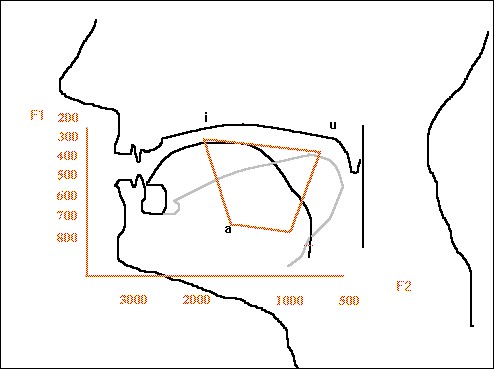
\includegraphics{picture/mouth.jpg}
\caption{vocal tract}
\end{figure}

\section{Methods}\label{methods}

\subsection{Participants}\label{participants}

Six female native (L1) Mandarin speakers and six female non-native (L2)
Mandarin speakers participated in the study. The mean age of the L1
Mandarin speakers is 22.33 (range: 23-30) and that of the L2 Mandarin
speakers is 26.33 (range: 18-28). Among L1 Mandarin speakers, two
speakers are from northern Mainland China (Beijing and Tianjin), three
speakers were from southern Mainland China (Nanjing, Chengdu and
Chongqing), and one speaker was from Taiwan. The Taiwanese participant
identified Mandarin as her most fluent language. All the six L2 Mandarin
speakers' native language was American English. They were all novice-low
learners who enrolled in first-year accelerated Chinese language course
at the same university. They had learned Mandarin for six months and
none of them had any study-abroad experience.

\subsection{Speech materials}\label{speech-materials}

We prepared nine Chinese sentences for speech materials. Each sentence
includes one of the following nine vowels: {[}i{]}, {[}y{]}, {[}u{]},
{[}e{]}, {[}o{]}, {[}ə{]}, {[}\ipatext{ɤ}{]}, {[}a{]},
{[}\ipatext{ɑ}{]}. Each vowel appears after the aspirated bilabial stop
{[}p{]} with a high tone (55).

\subsection{Procedure}\label{procedure}

Productions were elicited in a sentence-repetition oral task. Non-native
speakers (NNS) and native Chinese speakers (NS) were asked to read the
sentences twice. All participants read the speech materials for practice
once before recording. Recordings were made in a quiet study room in the
library using Praat Sound Recorder with 44,100 Hz sampling frequency,
and then these recordings were saved as wav files on a laptop. Formant 1
(F1) and Formant 2 (F2) were measured in the vowel mid-point for each
vowel shown in the spectrogram. All measurement was conducted using
Praat program on the same laptop. After the measurement, the mean F1 and
F2 values were plotted in charts using the program R to generate vowel
distribution for each speaker.

\section{Results and discussion}\label{results-and-discussion}

\subsection{Native speaker patterns}\label{native-speaker-patterns}

Table 1 shows the mean F1 and F2 values of nine Chinese vowels for
native speakers. Regarding F2 values, data shows that {[}i{]} had the
highest F2 values for all native speakers, and {[}u{]} had the lowest F2
values for NS2 and NS3, but not for NS1. As for F1 values, three NS also
had different lowest and highest values. While {[}i{]} had the lowest F1
value and {[}\ipatext{ɑ}{]} had the highest F1 value for NS1 and NS3,
NS2's {[}y{]} had the lowest F1 value and her {[}a{]} had the highest F1
value.

\begin{Shaded}
\begin{Highlighting}[]
\FunctionTok{\textbackslash{}newfontfamily\textbackslash{}ipa}\NormalTok{\{Doulos SIL\} }
\end{Highlighting}
\end{Shaded}

\begin{table}

\caption{\label{tab:table1}Formant by volwels among non-native and native groups}
\centering
\begin{tabular}[t]{llrrrr}
\toprule
group & vowel & F1\_mean & F2\_mean & F1\_sd & F2\_sd\\
\midrule
NNS & a & 913.33 & 1513.83 & 47.14 & 161.28\\
NNS & ɑ & 901.50 & 1377.00 & 63.86 & 107.69\\
NNS & e & 520.67 & 2320.00 & 65.50 & 95.07\\
NNS & ə & 651.33 & 1980.00 & 88.59 & 166.70\\
NNS & ɤ & 640.33 & 1702.33 & 70.43 & 238.62\\
\addlinespace
NNS & i & 335.67 & 2646.50 & 46.03 & 100.61\\
NNS & o & 551.50 & 1043.67 & 49.79 & 61.90\\
NNS & u & 416.00 & 1122.83 & 69.62 & 196.96\\
NNS & y & 321.50 & 1806.83 & 31.25 & 186.00\\
NS & a & 910.33 & 1655.50 & 115.38 & 142.20\\
\addlinespace
NS & ɑ & 848.00 & 1305.17 & 59.50 & 147.96\\
NS & e & 556.83 & 2486.50 & 38.02 & 128.39\\
NS & ə & 717.67 & 1850.50 & 40.10 & 101.96\\
NS & ɤ & 596.83 & 1289.67 & 105.92 & 152.62\\
NS & i & 308.33 & 2916.17 & 30.23 & 73.78\\
\addlinespace
NS & o & 554.50 & 908.67 & 48.53 & 76.63\\
NS & u & 335.00 & 840.00 & 15.63 & 56.02\\
NS & y & 309.17 & 2420.83 & 15.17 & 237.25\\
\bottomrule
\end{tabular}
\end{table}

Clearer vowel distribution for each native speaker can be seen in the
formant plots (Figure 1-3). According to the ``vowel dispersion
principle'', the vowel quadrilateral can be viewed as ``a perceptual
space in which vowels are located in the oral cavity'' (Ashby and
Maidment, 2005). In this study, the vowel quadrilateral is shown as
formant plots where the Y-axis is F1 (Hz) that corresponds to the height
of the tongue position; while the X-axis is F2 (Hz) that indicates the
backness of the tongue position for each vowel (Figure 1-3).

\begin{figure}
\centering
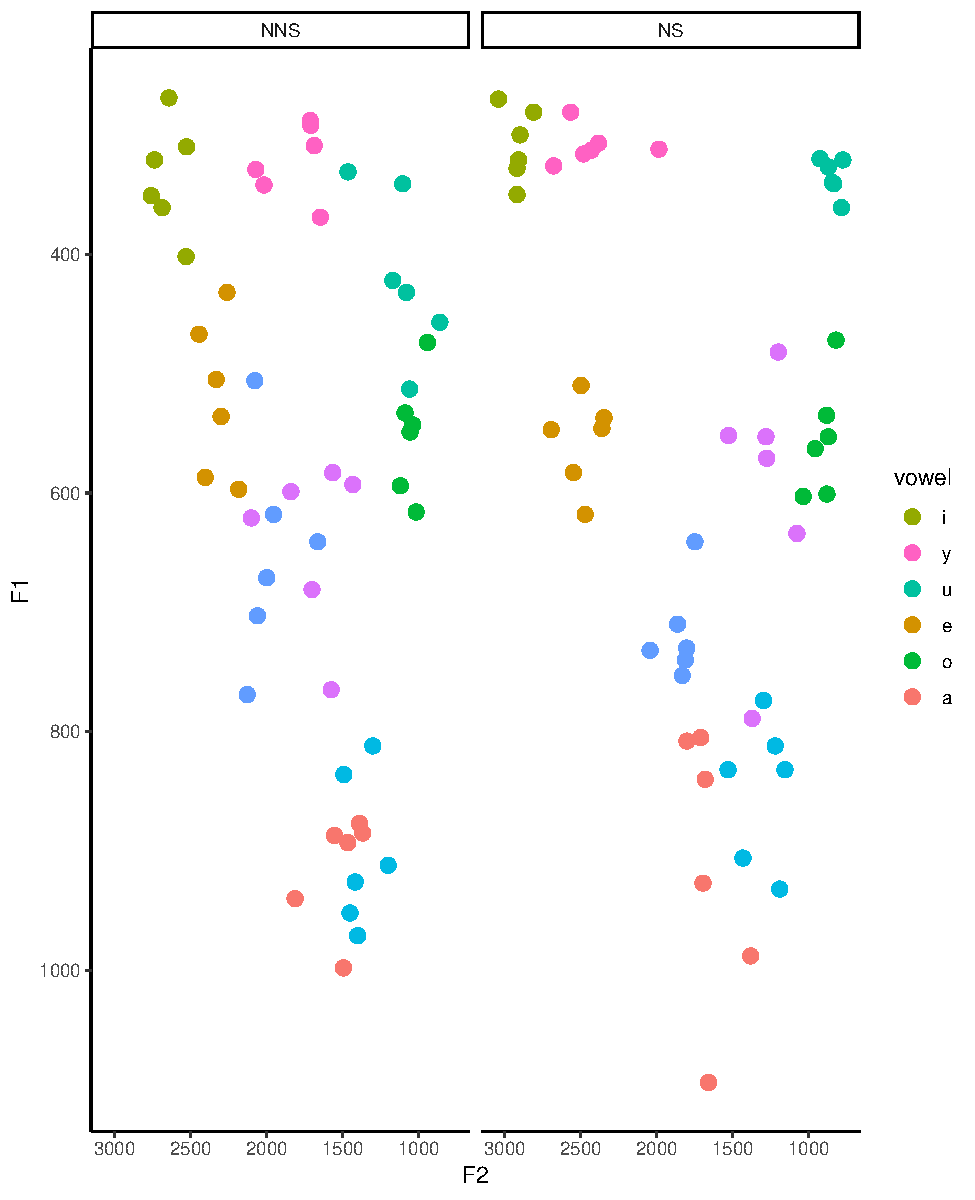
\includegraphics{Vowel_v3_files/figure-latex/figure1-1.pdf}
\caption{}
\end{figure}

\begin{figure}
\centering
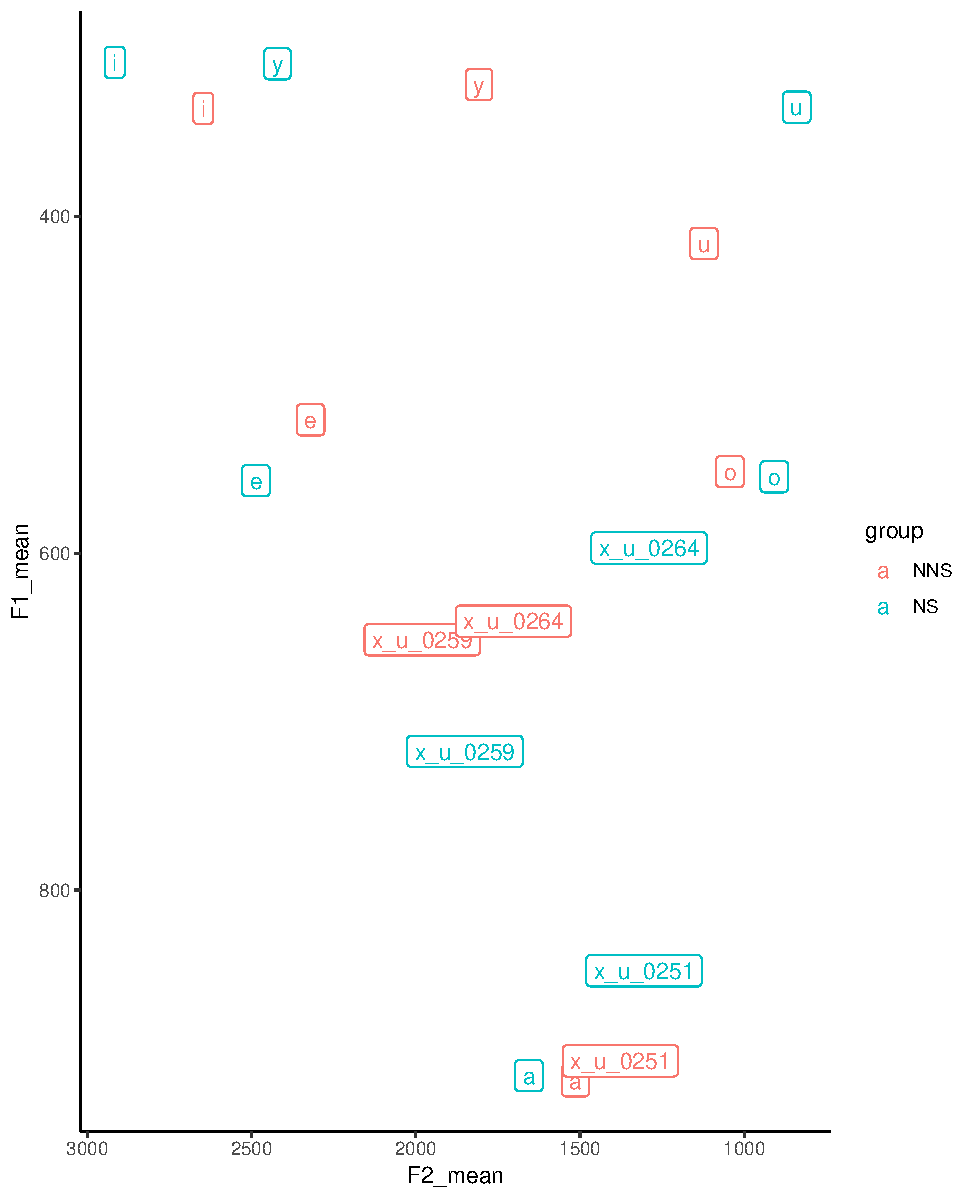
\includegraphics{Vowel_v3_files/figure-latex/figure2-1.pdf}
\caption{}
\end{figure}

\begin{figure}
\centering
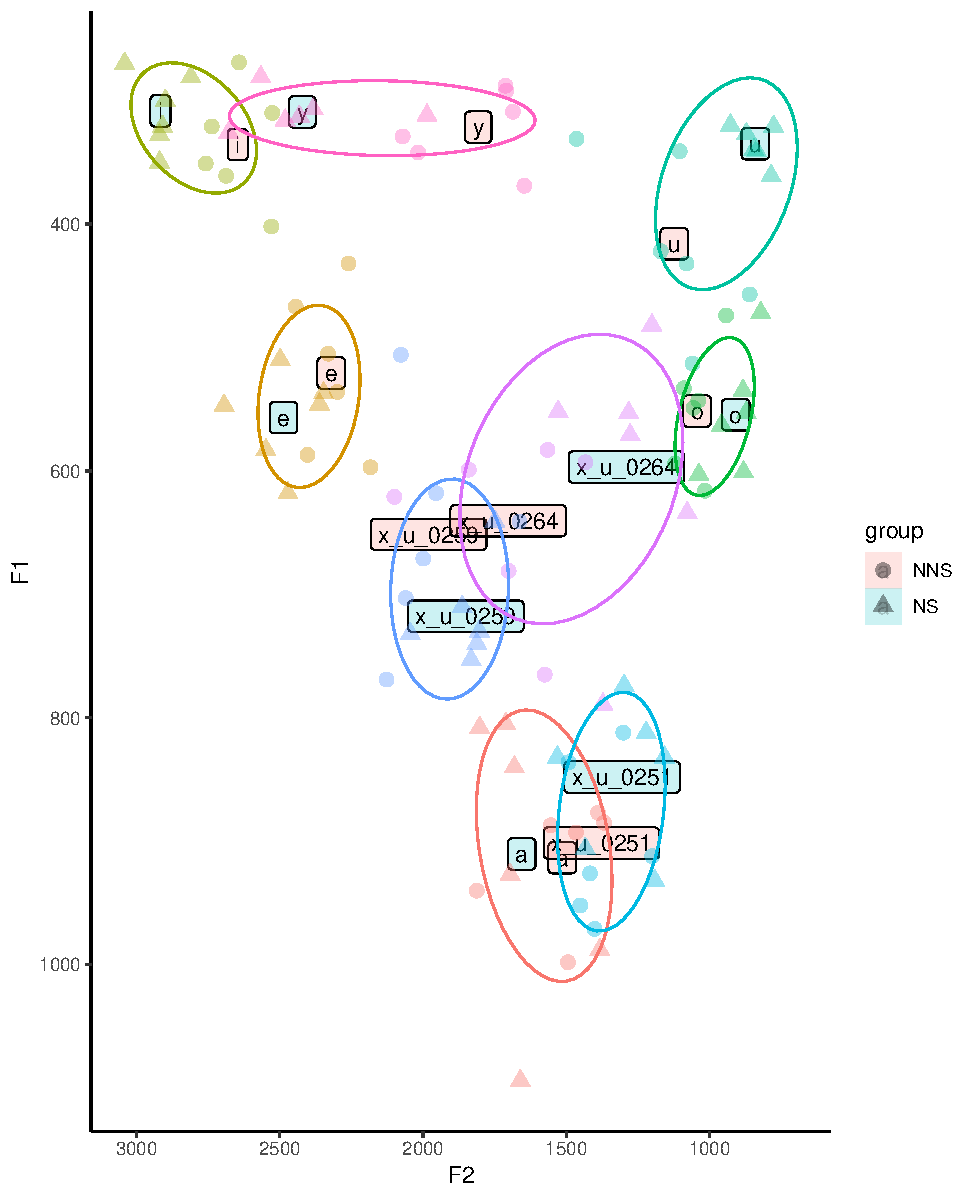
\includegraphics{Vowel_v3_files/figure-latex/figure3-1.pdf}
\caption{}
\end{figure}

\subsection{Second language
examination}\label{second-language-examination}

\section{Conclusion}\label{conclusion}

\newpage

\section{References}\label{references}

\begingroup
\setlength{\parindent}{-0.5in} \setlength{\leftskip}{0.5in}

\hypertarget{refs}{}
\hypertarget{ref-ashby2005}{}
Ashby, M., \& Maidment, J. (2005). \emph{Introducing phonetic science}.
Cambridge University Press.

\hypertarget{ref-hinton2006}{}
Hinton, L., Nichols, J., \& Ohala, J. J. (2006). \emph{Sound symbolism}.
Cambridge University Press.

\hypertarget{ref-roach2004}{}
Roach, P. (2004). British english: Received pronunciation. \emph{Journal
of the International Phonetic Association}, \emph{34}(2), 239--245.

\endgroup

\begin{Shaded}
\begin{Highlighting}[]
\FunctionTok{\textbackslash{}newfontfamily\textbackslash{}ipa}\NormalTok{\{Doulos SIL\} }
\end{Highlighting}
\end{Shaded}


\end{document}
